\documentclass[11pt, a4paper]{article}

\usepackage[a4paper, margin=2.5cm]{geometry}
\usepackage[T1]{fontenc}
\usepackage[utf8]{inputenc}
\usepackage[english]{babel}

\usepackage{amsmath,amsfonts,amssymb}
\usepackage{graphicx}
\usepackage{hyperref}
\usepackage{enumitem}
\usepackage{booktabs}
\usepackage{animate}

\title{\textbf{Lecture Notes: Attention and Transformers}\\ \Large AI in Practice (MSc Informatics)}

\begin{document}
\maketitle

\tableofcontents
\newpage

\section{Introduction}

These lecture notes provide a comprehensive overview of the Transformer architecture, the foundational model for modern Artificial Intelligence and Natural Language Processing. We will explore the motivations behind moving away from recurrent models, dive deep into tokenization and embeddings, deconstruct the self-attention mechanism, and survey modern architectures and alignment techniques. This material was made with AI.

\section{Sequence Modeling and Motivation}

To appreciate the design of the Transformer, we must first understand the problem it was built to solve. Sequence-to-sequence tasks---such as translating a sentence from English to Hungarian, summarizing a long document, or generating code---require a model to process an input sequence of tokens and produce an output sequence. 

\subsection{The Recurrent Bottleneck}
Historically, sequence modeling was dominated by Recurrent Neural Networks (RNNs) and their more advanced variants like Long Short-Term Memory (LSTM) networks. RNNs process tokens strictly sequentially: to understand the 10th word in a sentence, the network must first process words 1 through 9, updating a ``hidden state'' at each step. 

While theoretically sound, this sequential nature introduced two massive bottlenecks:
\begin{itemize}[leftmargin=*]
    \item \textbf{Loss of Context:} In long sequences, the hidden state becomes an information bottleneck. By the time the RNN reaches the 50th word, it has often "forgotten" the critical context provided by the 1st word.
    \item \textbf{Lack of Parallelization:} Because step $t$ depends on step $t-1$, RNNs cannot be parallelized across the tokens of a sequence. Modern GPUs are designed for massive parallel computation; RNNs leave this hardware largely idle.
\end{itemize}

\begin{figure}[ht]
\centering
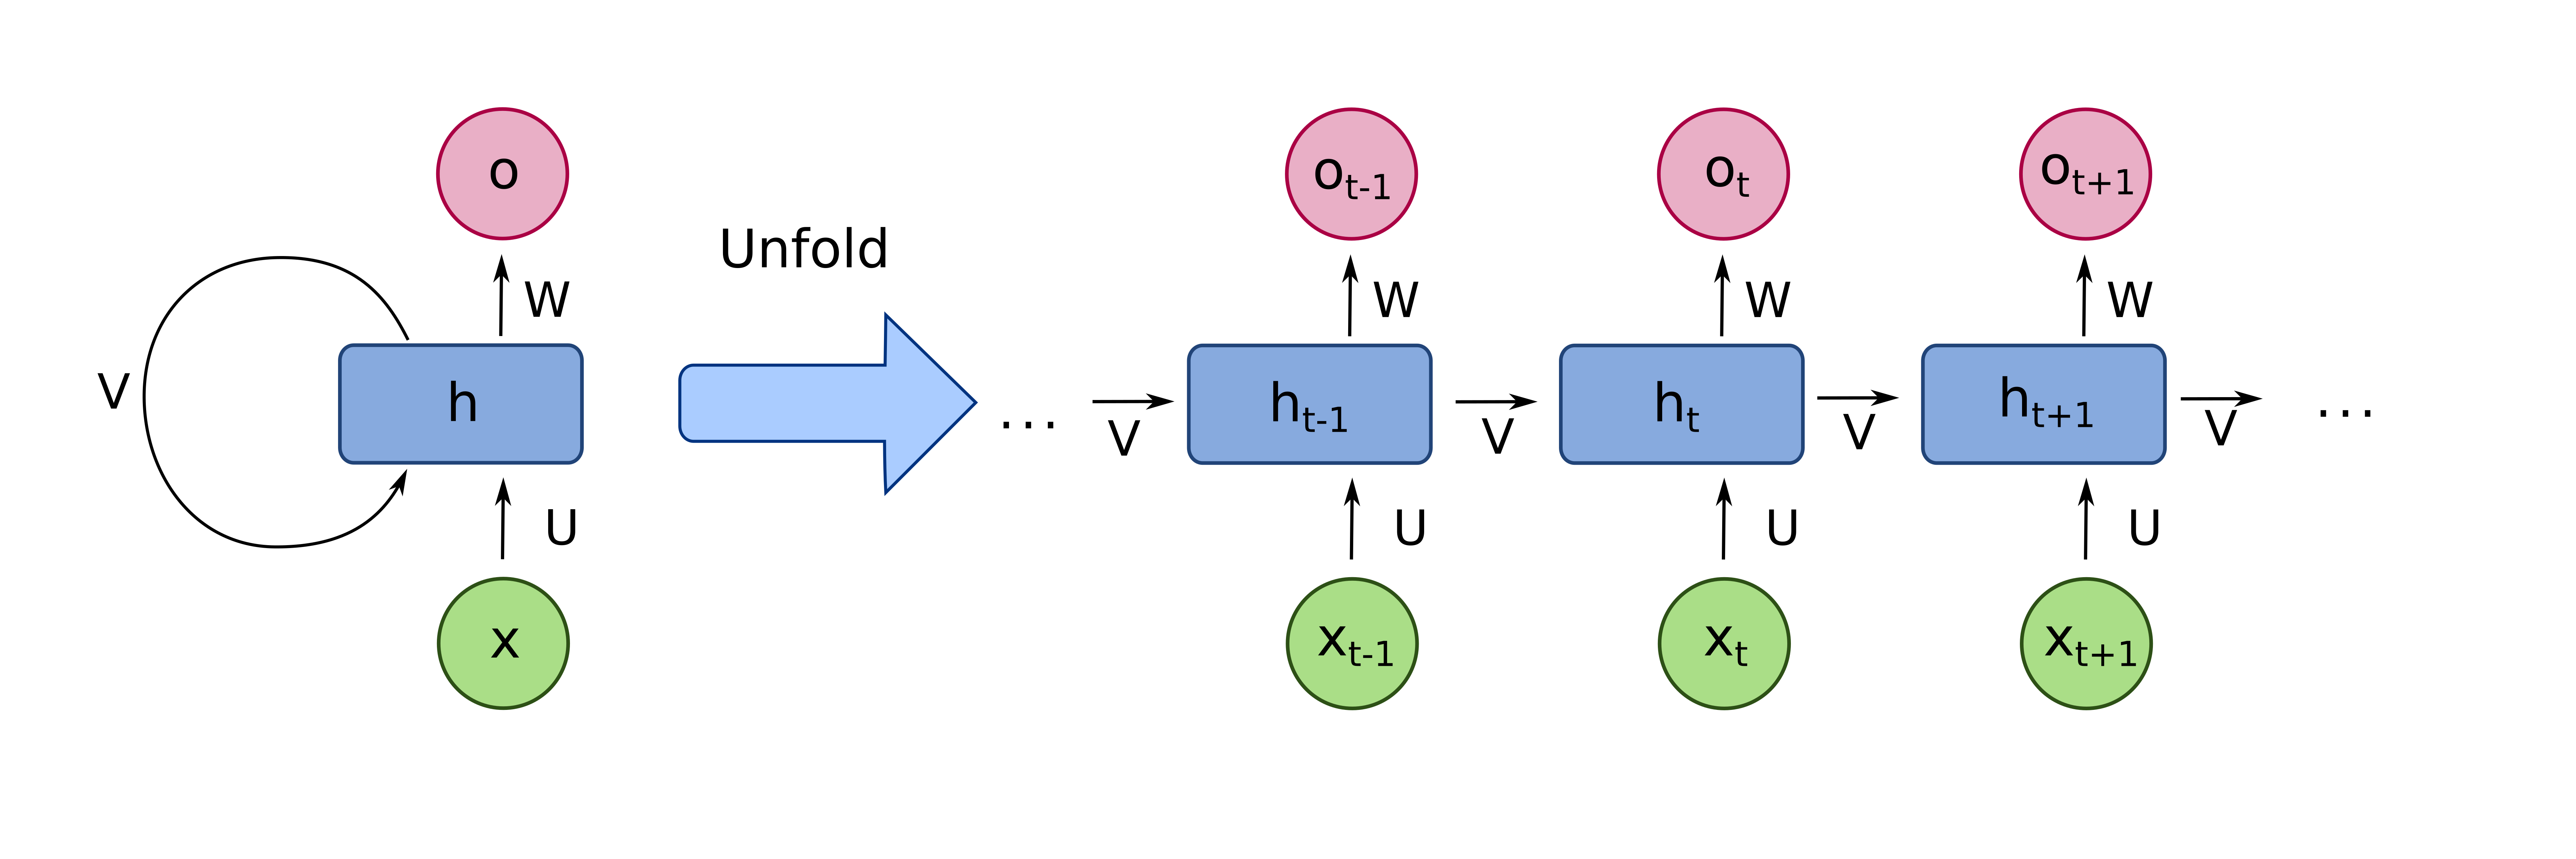
\includegraphics[width=0.8\linewidth]{Recurrent_neural_network_unfold.png}
\caption{An unrolled RNN demonstrates the sequential dependency problem: state $h_t$ strictly requires the computation of $h_{t-1}$. (Image: \href{https://commons.wikimedia.org/wiki/File:Transformer,_full_architecture.png}{fdeloche}, \href{https://creativecommons.org/licenses/by-sa/4.0/}{CC BY 4.0})}
\label{fig:rnn}
\end{figure}

\subsection{The Introduction of Attention}
To solve the ``forgetting'' problem, Bahdanau \textit{et al.} (2015) introduced the concept of \textbf{Attention} in sequence-to-sequence models. Instead of forcing the entire input sequence into a single hidden vector, the model was allowed to ``look back'' at all previous hidden states and assign different weights (attention) to different words depending on what it was trying to generate at the current step. 

\subsection{Attention Is All You Need}
In 2017, Vaswani \textit{et al.} published the groundbreaking paper \textit{Attention Is All You Need}. They asked a simple question: if attention is the key to solving long-range dependencies, do we need the slow, sequential RNN at all? Their answer was the \textbf{Transformer}, an architecture that threw away recurrence entirely. By using \textit{self-attention}, the Transformer processes all tokens in a sequence simultaneously, evaluating the relationship between every pair of words in parallel. This unblocked the ability to train on massive datasets, directly leading to the era of Large Language Models (LLMs).

\section{Tokenization}

Before a neural network can process text, the text must be converted into numbers. This process is called tokenization. Tokenization strategies profoundly affect model performance, memory usage, and the ability to handle rare words.

\subsection{Granularity of Tokenization}
There are three primary philosophies for breaking down text:
\begin{enumerate}
    \item \textbf{Word-level:} Splitting by spaces and punctuation. \textit{Pros:} Intuitively meaningful tokens. \textit{Cons:} Results in massive vocabularies. If ``run'', ``runs'', and ``running'' are separate tokens, the model struggles to generalize. Furthermore, Out-Of-Vocabulary (OOV) words break the model.
    \item \textbf{Character-level:} Treating every letter as a token. \textit{Pros:} Tiny vocabulary (e.g., 256 ASCII characters), no OOV issues. \textit{Cons:} Sequences become extremely long, drastically slowing down the Transformer, and characters lack inherent semantic meaning.
    \item \textbf{Subword-level:} The modern standard. Common words (like ``dog'') remain intact, while rare or complex words (like ``unbelievable'') are broken into logical subword chunks (e.g., ``un'', ``believ'', ``able'').
\end{enumerate}

\subsection{Byte-Pair Encoding (BPE): A Step-by-Step Example}
Most modern LLMs (including the GPT family) use a subword algorithm called Byte-Pair Encoding (BPE). BPE is a data compression technique adapted for NLP. 

Imagine a training corpus with the following word frequencies:
\begin{itemize}
    \item \texttt{low}: 5
    \item \texttt{lower}: 2
    \item \texttt{newest}: 6
    \item \texttt{widest}: 3
\end{itemize}

BPE starts with a character-level vocabulary: \texttt{l, o, w, e, r, n, s, t, i, d}. It then iteratively merges the most frequent adjacent pair of tokens:
\begin{enumerate}
    \item The pair \texttt{e} and \texttt{s} appears most frequently (in \texttt{newest} and \texttt{widest}, total $6+3=9$ times). We merge them to create a new token: \texttt{es}.
    \item Next, \texttt{es} and \texttt{t} appear together 9 times. We merge them to create \texttt{est}.
    \item The pair \texttt{l} and \texttt{o} appears 7 times (\texttt{low} and \texttt{lower}). We merge them to \texttt{lo}.
\end{enumerate}
This process repeats until a target vocabulary size (e.g., 50,000 tokens) is reached. 

\subsection{Special Tokens}
Tokenizers also introduce artificial tokens for structural purposes. Examples include \texttt{[CLS]} (used to aggregate sequence representations for classification), \texttt{[SEP]} (to separate sentences), and \texttt{[PAD]} (to pad shorter sequences in a batch to a uniform length). 

For example, the phrase \emph{``I love transformers!''} might be tokenized and mapped to integer IDs as follows:
\{``I'', ``love'', ``trans'', ``\texttt{\#\#form}'', ``\texttt{\#\#ers}'', ``!''\} $\rightarrow$ \{12, 45, 1023, 2567, 89, 3\}. Trade-offs are clear: a larger vocabulary lowers the token count (allowing longer text context) but dramatically increases the size of the embedding matrix.

\section{Vector Embeddings}

Once we have integer token IDs, the network must convert them into a continuous mathematical space. Each token ID maps to a learnable dense vector called an \textbf{embedding}. 

\subsection{The Semantic Space}
If we use an embedding dimension of $d=768$, each word is represented by a coordinate in a 768-dimensional space. The remarkable property of these learned embeddings is that they capture semantic meaning. Words with similar meanings (e.g., "cat" and "pet") are moved closer together during training. 

\begin{figure}[ht]
\centering
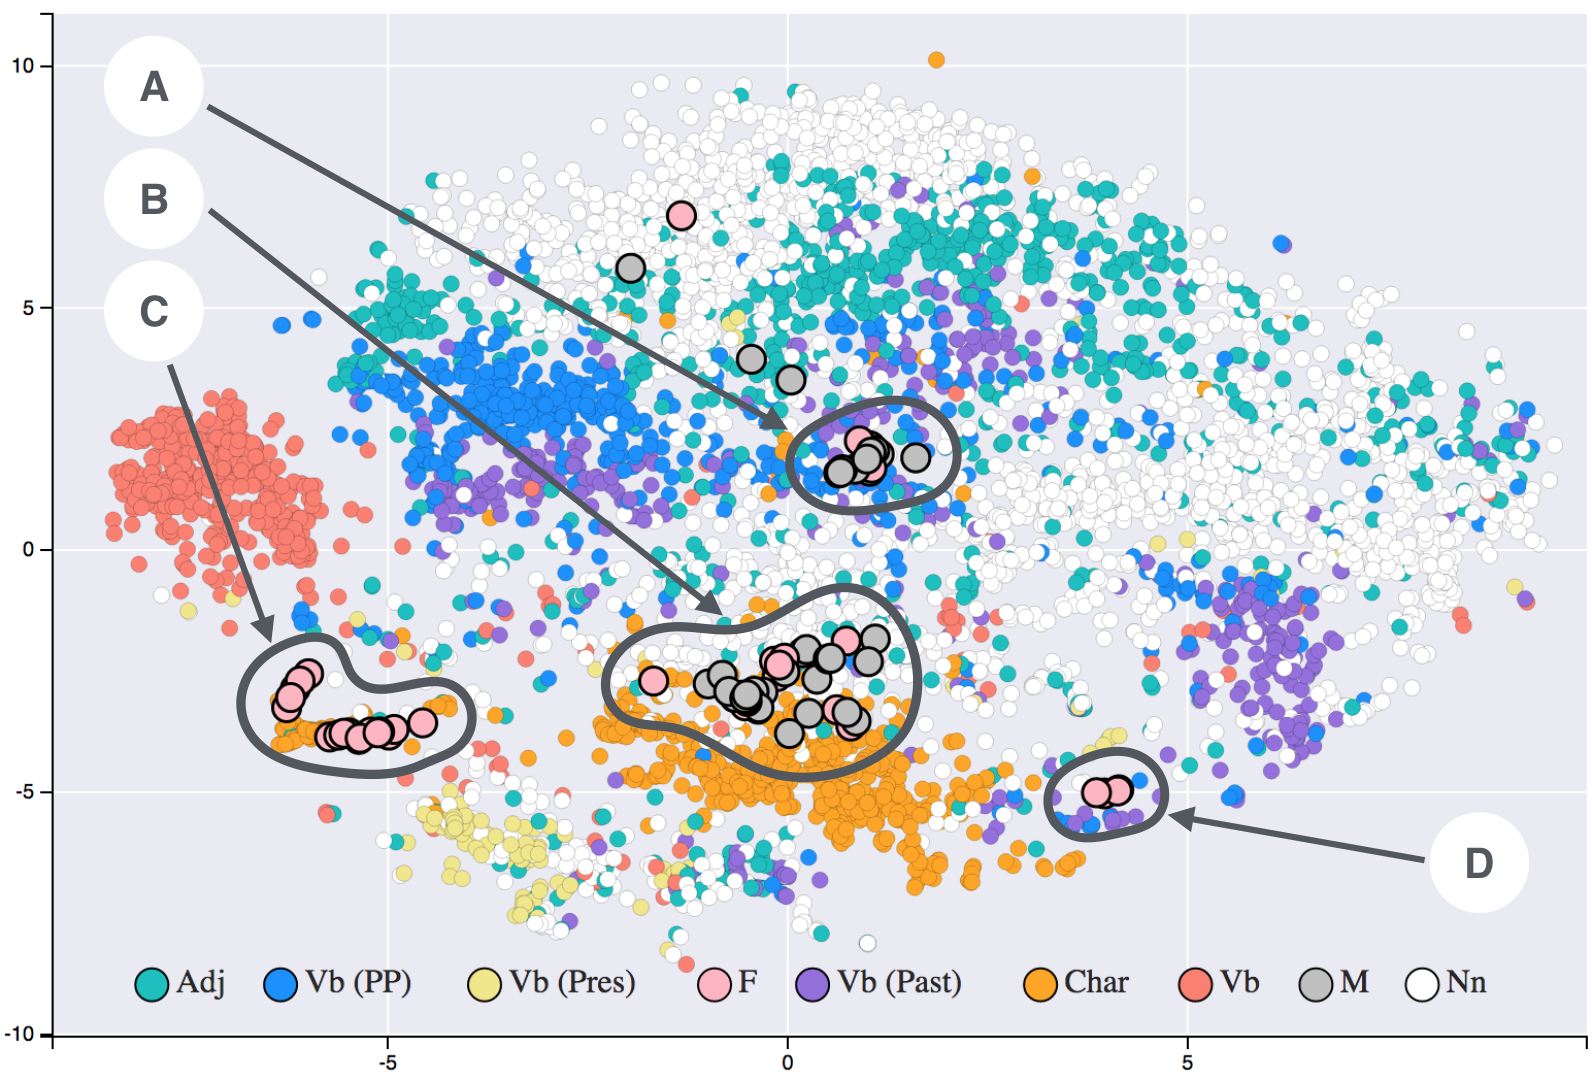
\includegraphics[width=0.7\linewidth]{vector_embeddings.png}
\caption{Example 2D projection of learned word embedding vectors (t-SNE of a historical text corpus). Nearby points tend to be related words (e.g., grouped adjectives or verbs). Notice how syntactic and semantic properties cluster naturally. (Image: \href{https://commons.wikimedia.org/wiki/File:T-SNE_visualisation_of_word_embeddings_generated_using_19th_century_literature.png}{Siobhán Grayson}, \href{https://creativecommons.org/licenses/by-sa/4.0/}{CC BY 4.0})}
\label{fig:embeddings}
\end{figure}

Furthermore, relationships become mathematical vectors. The famous Word2Vec example showed that the vector distance between ``King'' and ``Queen'' is roughly the same as the distance between ``Man'' and ``Woman''. 

\subsection{Static vs. Contextual Embeddings}
It is crucial to distinguish between the \textit{input} embeddings and the \textit{contextual} representations that emerge later in the network.
\begin{itemize}
    \item \textbf{Static Embeddings:} The initial lookup table. The token ``bank'' gets the exact same vector whether it is in the context of a ``river bank'' or a ``financial bank''.
    \item \textbf{Contextual Embeddings:} As the vector passes through the Transformer's self-attention layers, it absorbs context from surrounding words. By the final layer, the representation for ``bank'' in ``river bank'' will be entirely different from ``financial bank''.
\end{itemize}

\section{Embedding Lookup and One-Hot Equivalence}

How do we actually retrieve these vectors? Mathematically, embedding lookup is often described as a matrix multiplication with a one-hot encoded vector.

Let $V$ be the vocabulary size (e.g., 50,000) and $d$ be the embedding dimension (e.g., 768). Our embedding matrix $E$ has shape $V \times d$.
Suppose we want the embedding for token ID 3. We can represent token ID 3 as a one-hot vector $e_3 = [0, 0, 1, 0, \dots, 0]$ of size $1 \times V$. 

If we multiply $e_3$ by $E$:
$$ \text{Embedding} = e_3 \times E $$
The rules of matrix multiplication dictate that this operation simply extracts the 3rd row of the matrix $E$. 

In practical implementations (like PyTorch or TensorFlow), creating a massive vector of 49,999 zeros and a single 1 is a waste of memory. Instead, deep learning frameworks use highly optimized \textbf{gather} operations, functioning essentially as a hash map or array index lookup, directly grabbing the $i$-th row.

The total number of parameters in the embedding matrix is large ($V \times d$). To save parameters, models often use \textbf{weight tying}, where the output layer (which projects the final $d$-dimensional representation back into a $V$-dimensional space to predict the next word) shares the exact same weights as the input embedding matrix.

\section{Positional Information}

RNNs inherently know the order of sequences because they process data one token at a time. The Transformer, however, receives the entire sequence at once. If we simply feed token embeddings into self-attention, the model treats the sequence as an unordered ``bag of words''. The sentence ``The dog bit the man'' would look identical to ``The man bit the dog''. We must inject positional information.

\subsection{Sinusoidal Positional Encodings}
In the original Transformer, Vaswani \textit{et al.} created a set of static positional vectors that are added element-wise to the token embeddings. They used sine and cosine functions of different frequencies:
$$ PE_{p,2i} = \sin\left(\frac{p}{10000^{2i/d}}\right) $$
$$ PE_{p,2i+1} = \cos\left(\frac{p}{10000^{2i/d}}\right) $$
where $p$ is the position in the sequence, $i$ is the dimension index, and $d$ is the embedding dimension.

\textbf{Intuition:} Think of this like the hands of a clock. The last dimensions (the ``hour hand'') change very slowly as you move through a document. The middle dimensions (the ``minute hand'') change moderately. The first dimensions (the ``second hand'') fluctuate rapidly back and forth between every token. Together, they create a unique, continuous ``time signature'' for every position.

\subsection{Modern Relative Positional Encodings}
Absolute positions (token 1, token 2) are less important than relative positions (token X is 3 words away from token Y). Modern models have largely moved to relative encodings:
\begin{itemize}
    \item \textbf{Rotary Positional Embeddings (RoPE):} Used by LLaMA and others. Instead of adding a vector, RoPE applies a mathematical rotation to the token vectors in 2D space based on their position. The dot product between two rotated vectors naturally encodes their relative distance.
    \item \textbf{ALiBi (Attention with Linear Biases):} Instead of changing the embeddings at all, ALiBi subtracts a penalty directly from the final attention score between two words, proportional to how far apart they are. This requires no extra parameters and extrapolates exceptionally well to longer texts than the model was trained on.
\end{itemize}

\section{Attention: Query, Key, Value}

This is the core engine of the Transformer. To understand self-attention, it is best to use an information retrieval analogy (like searching a library database).

Imagine you go to a library looking for a book. 
\begin{itemize}
    \item Your search term is the \textbf{Query} (Q). 
    \item Every book in the library has a title and metadata, which acts as the \textbf{Key} (K).
    \item The actual content of the book is the \textbf{Value} (V).
\end{itemize}
You compare your Query to every Key. The more similar they are, the higher the score. You then retrieve the Values weighted by those scores.

In a Transformer, \textit{every token acts as all three}. For a specific word in a sentence, it formulates a Query (what context it is looking for), it provides a Key (what information it contains), and it offers a Value (its actual semantic payload).

\subsection{The Mathematical Steps}
The model maintains three learned weight matrices: $W^Q, W^K, W^V$. The input embeddings are multiplied by these matrices to produce $\mathbf{q}$, $\mathbf{k}$, and $\mathbf{v}$ vectors for each token.

The process of \textbf{Scaled Dot-Product Attention} is defined as:
$$ \text{Attention}(Q, K, V) = \text{softmax}\left(\frac{Q K^T}{\sqrt{d_k}}\right) V $$

Let's break this down step-by-step:
\begin{enumerate}
    \item \textbf{Dot Product ($QK^T$):} We take the dot product of every Query with every Key. This results in an $N \times N$ similarity matrix (where $N$ is sequence length). High scores mean high relevance.
    \item \textbf{Scaling ($\frac{1}{\sqrt{d_k}}$):} If the vector dimension $d_k$ is large, dot products can yield massive numbers. This pushes the softmax function into regions with near-zero gradients. Dividing by the square root of the dimension stabilizes the training.
    \item \textbf{Softmax:} We apply softmax to each row of the matrix. This converts the raw scores into a probability distribution (all weights between 0 and 1, summing to 1). 
    \item \textbf{Weighting Values ($\times V$):} We multiply these softmax probabilities by the Value matrix. If Token 1 strongly attended to Token 4 (weight 0.9), Token 1's new representation will be heavily composed of Token 4's Value.
\end{enumerate}

\begin{figure}[ht]
\centering
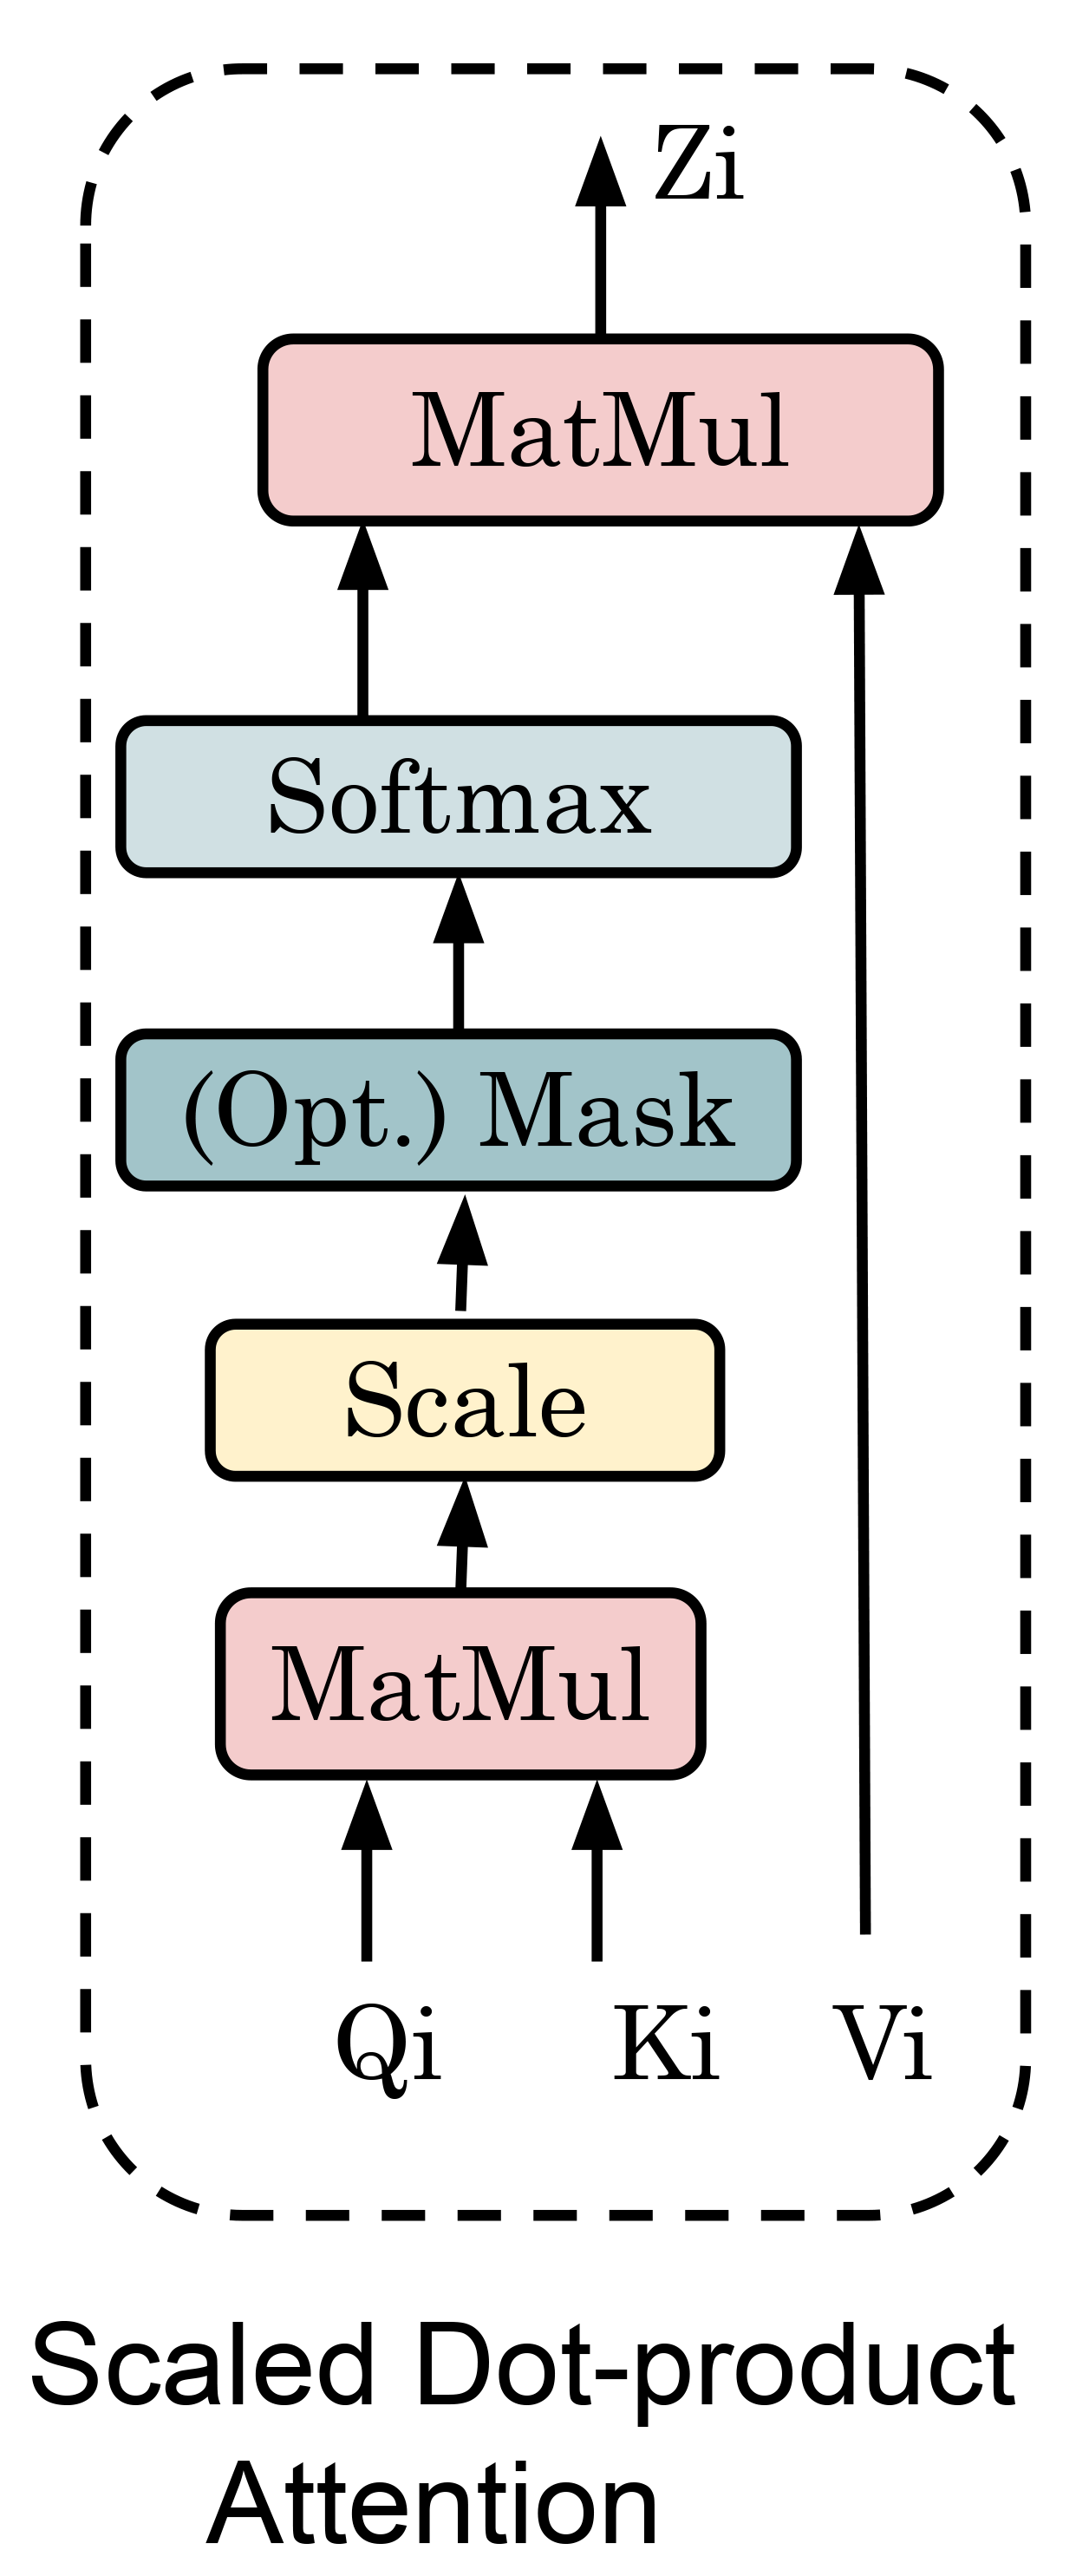
\includegraphics[scale=0.25]{attention_diagram.png}
\caption{The components of Scaled Dot-Product Attention: MatMul, Scale, Masking, Softmax, and a final MatMul. (Image: \href{https://commons.wikimedia.org/wiki/File:Self-Attention_(Scaled_dot-product_Attention).png}{https://arxiv.org/abs/2307.07982}, \href{https://creativecommons.org/licenses/by-sa/4.0/}{CC BY 4.0})}
\label{fig:attention_diagram}
\end{figure}

\subsection{Causal Masking}
In tasks like language generation, a token is not allowed to ``look into the future'' to predict the next word. We enforce this by applying a \textbf{causal mask} to the $QK^T$ matrix before the softmax step. All positions corresponding to future tokens are overwritten with $-\infty$. When passed through softmax, $e^{-\infty} = 0$, ensuring the model strictly attends only to past and present tokens.

\section{Multi-Head Attention}

A single sentence contains multiple layers of relationships. Consider: \emph{``The exhausted student handed the completed assignment to the professor.''} 
The word \emph{``handed''} relates to \emph{``student''} (who did the handing), \emph{``assignment''} (what was handed), and \emph{``professor''} (to whom).

A single attention mechanism might struggle to capture all these distinct relationships simultaneously. \textbf{Multi-Head Attention} solves this by splitting the vector dimension $d_{model}$ into $h$ independent "heads". If $d_{model} = 768$ and $h=12$, each head operates in a 64-dimensional subspace.

Each head independently performs the complete Q-K-V attention mechanism with its own uniquely learned weights. 
\begin{itemize}
    \item Head 1 might learn to track grammatical subjects.
    \item Head 2 might learn to track coreferences (what a pronoun refers to).
    \item Head 3 might act strictly locally, just looking at the immediately preceding word.
\end{itemize}
Finally, the outputs from all $h$ heads are concatenated back into a single vector of size $d_{model}$ and pushed through a final linear layer to mix the learned information.

\section{Transformer Architectures}

While the fundamental blocks remain the same, they can be assembled differently based on the task. The original 2017 paper proposed an \textbf{Encoder-Decoder} structure for translation, but the field has since split into three primary architectural families.

\begin{figure}[ht]
\centering
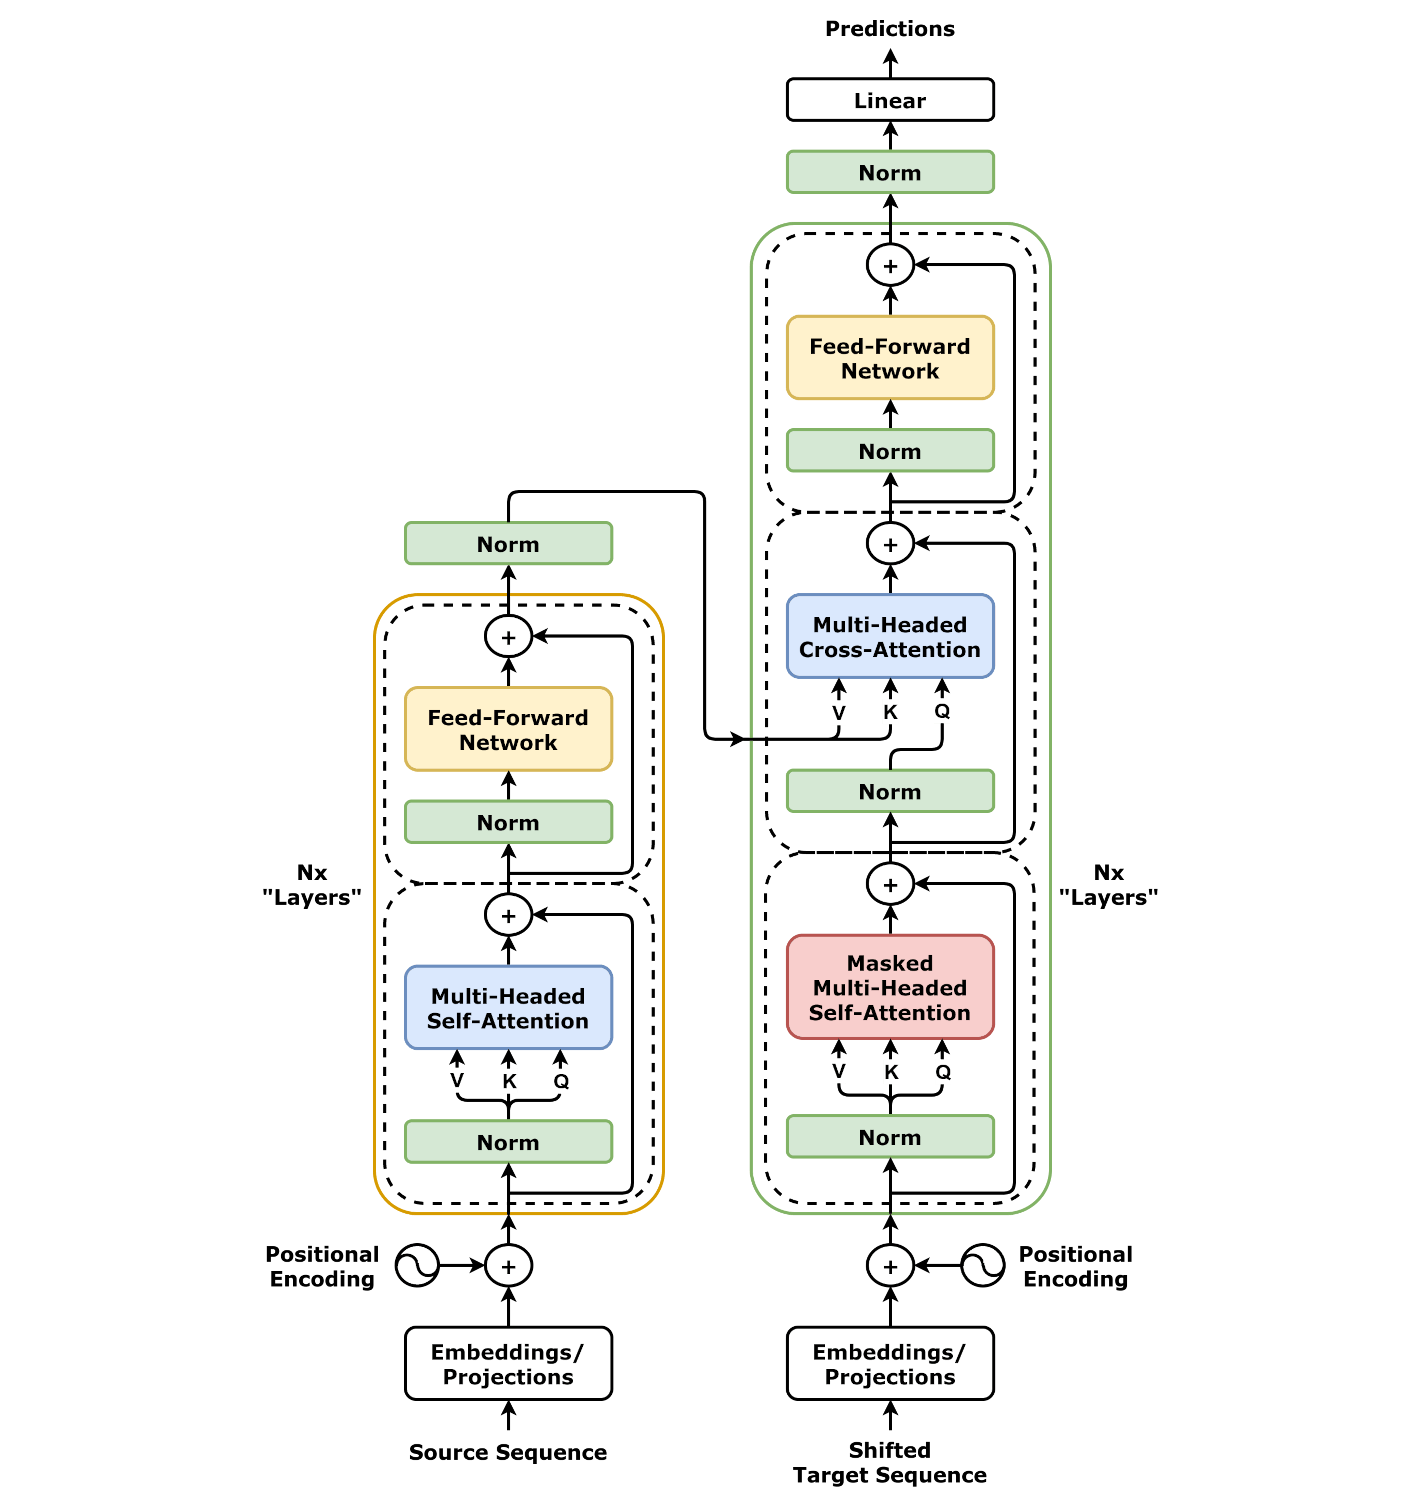
\includegraphics[scale=0.25]{transformer_stacked_layers.png}
\caption{The original Transformer architecture features a stacked encoder (left) and decoder (right). The encoder extracts bidirectional context, while the decoder generates autoregressively, attending both to its own past and the encoder's outputs. (Image: \href{https://commons.wikimedia.org/wiki/File:Transformer,_full_architecture.png}{dvgodoy}, \href{https://creativecommons.org/licenses/by-sa/4.0/}{CC BY 4.0}).}
\label{fig:transformer}
\end{figure}

\subsection{Encoder-Only Models (e.g., BERT, RoBERTa)}
Encoder models use bidirectional self-attention—every token can see every other token in the sequence (no causal masking). This makes them incredibly powerful at understanding the deep context of a text.
\begin{itemize}
    \item \textbf{Use Cases:} Sentiment analysis, named entity recognition, document classification, extractive question answering.
    \item \textbf{Limitation:} They cannot easily generate new text word-by-word.
\end{itemize}

\subsection{Decoder-Only Models (e.g., GPT-3, LLaMA, Mistral)}
Decoder models use strictly causally-masked self-attention. A token can only look backwards. Though seemingly a handicap for basic understanding, when scaled up, this architecture has proven universally capable.
\begin{itemize}
    \item \textbf{Use Cases:} Autoregressive text generation, chat assistants, code generation.
    \item \textbf{Advantage:} Highly streamlined, mathematically simpler to train at massive scale, naturally suited to open-ended generation.
\end{itemize}

\subsection{Encoder-Decoder Models (e.g., T5, BART)}
Retaining the original architecture, these models use an unmasked encoder to process an input, and a masked decoder to generate the output. The decoder contains a special \textbf{Cross-Attention} layer where the Queries come from the decoder, but the Keys and Values are piped in from the encoder.
\begin{itemize}
    \item \textbf{Use Cases:} Machine translation, text summarization (where the input is fully available, and the output must be dynamically generated based on it).
\end{itemize}

\section{Training Objectives and Inference}

How do we actually train these billions of parameters? Depending on the architecture, different self-supervised training objectives are utilized on massive corpora of text (like the entire internet).

\subsection{Pre-Training Objectives}
\begin{itemize}
    \item \textbf{Masked Language Modeling (MLM):} Used for Encoders (BERT). The tokenizer randomly obscures 15\% of the input tokens with a \texttt{[MASK]} token. The model is forced to use the surrounding unmasked context to guess the missing word. 
    \item \textbf{Causal Language Modeling (CLM):} Used for Decoders (GPT). The model is given a sequence of words and must predict the highly probable next word. The loss is computed across every position simultaneously (shifting the input right by one to act as the target).
\end{itemize}

\subsection{Inference and Decoding Strategies}
During deployment (inference), generating text autoregressively requires deciding how to pick the next word from the final probability distribution.
\begin{itemize}
    \item \textbf{Greedy Search:} Simply picking the token with the highest probability. Fast, but often leads to repetitive or suboptimal, sterile text.
    \item \textbf{Beam Search:} Keeps track of the top $K$ most likely sentence paths concurrently. If picking a slightly less probable word now leads to a highly probable sequence of words later, Beam Search will find it. Heavily used in translation.
    \item \textbf{Top-K and Nucleus (Top-p) Sampling:} Instead of picking strictly the best, the model samples randomly from a restricted pool of the most likely words. This injects "creativity" and variance, vital for chatbots and creative writing. A "temperature" parameter controls how flat (random) or sharp (deterministic) this probability curve is.
\end{itemize}

\begin{figure}[htbp]
\centering
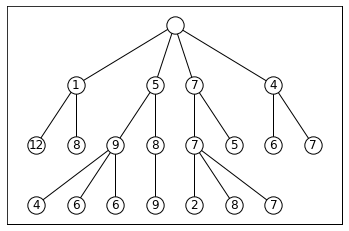
\includegraphics[width=0.43\linewidth]{frame-0.png}
    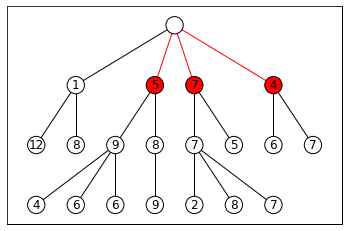
\includegraphics[width=0.43\linewidth]{frame-1.png}

    \vspace{0.5em}

    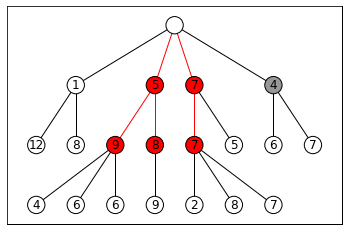
\includegraphics[width=0.43\linewidth]{frame-2.png}
    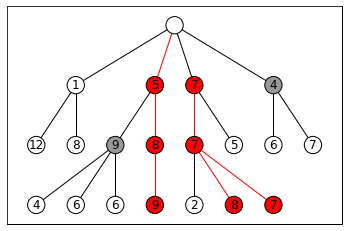
\includegraphics[width=0.43\linewidth]{frame-3.png}
\caption{Beam search explores multiple high-probability sequence branches simultaneously, preventing the model from getting stuck in local optima. (Image: \href{https://commons.wikimedia.org/wiki/File:Beam_search.gif}{BogdanShevchenko}, \href{https://creativecommons.org/licenses/by-sa/4.0/}{CC BY 4.0})}
\label{fig:beam_search}
\end{figure}

\section{Alignment: From Autocomplete to Assistant}

A model trained purely on Next Token Prediction on internet text is not a useful assistant. If you prompt it with \emph{"Write a poem about AI"}, it might just complete it with \emph{"Write a poem about space."} (acting like a forum autocomplete).

To bridge this gap, modern practice utilizes a pipeline of fine-tuning, commonly referred to as Alignment.

\subsection{Supervised Fine-Tuning (SFT)}
The model is trained on tens of thousands of high-quality human demonstrations. The data is structured purely as Prompt / Response pairs. This teaches the model the \textit{format} of being an assistant, answering questions directly instead of predicting random web-page continuations.

\subsection{Reinforcement Learning from Human Feedback (RLHF)}
Even with SFT, models can hallucinate or output unsafe content. RLHF addresses this:
\begin{enumerate}
    \item \textbf{Reward Model:} The SFT model generates multiple answers to a prompt. Humans rank these answers from best to worst. A separate "Reward Model" is trained to predict these human scores.
    \item \textbf{PPO Optimization:} The main language model generates responses, the Reward Model scores them, and the main model updates its weights using Proximal Policy Optimization (PPO) to maximize the reward score over time.
\end{enumerate}
This pipeline is what made models like ChatGPT uniquely conversational and helpful compared to their raw, pre-trained base models.

\section{Complexity and Practical Considerations}

Despite their power, Transformers have a severe computational Achilles' heel: the attention matrix.

\subsection{Quadratic Complexity}
Self-attention compares every token to every other token. If your sequence has $N$ tokens, the similarity matrix $QK^T$ has size $N \times N$. 
\begin{itemize}
    \item For 1,000 tokens, the matrix has 1,000,000 cells.
    \item For 10,000 tokens, it has 100,000,000 cells.
\end{itemize}
Both computation time and VRAM usage scale at $O(N^2)$. This is why early Transformers were limited to strict 512-token context windows. 

\subsection{Key-Value (KV) Caching}
During inference, a GPT model generates one word, appends it to the input, and runs the whole sequence again to get the next word. Recomputing the Key and Value matrices for the past words (which haven't changed) is a massive waste of FLOPS. 
Modern inference engines cache the K and V matrices of all previous tokens in memory. When predicting token $t$, the model only computes Q, K, V for token $t$, and fetches the rest from RAM. While this saves compute, the KV Cache grows sequentially, eventually becoming a massive memory bottleneck for long chats.

\section{Modern Variants and Improvements}

The field has iterated rapidly since 2017. Here are a few essential modern advancements defining current state-of-the-art models:

\begin{itemize}[leftmargin=*]
  \item \textbf{FlashAttention (Dao \textit{et al.}, 2022):} A revolutionary hardware-aware implementation of exact attention. Standard attention writes the massive $N \times N$ matrix to GPU memory (HBM) repeatedly. FlashAttention tiles the computation, keeping the matrix fragments entirely inside the ultra-fast GPU SRAM. This is not an approximation; it yields the exact same mathematical result but drastically reduces memory usage and speeds up training.
  \item \textbf{Mixture of Experts (MoE):} Used in models like Mixtral and GPT-4. Instead of every token passing through all parameters in a layer, a router network selectively assigns tokens to specialized "expert" sub-networks. A 47-billion parameter MoE model might only use 12 billion parameters during any single forward pass, providing the performance of a massive model at the inference cost of a smaller one.
  \item \textbf{Grouped-Query Attention (GQA):} To solve the KV-Cache memory explosion, modern architectures (like LLaMA 2 and 3) don't give every attention head its own unique K and V projections. Instead, multiple Query heads share a single Key/Value head. This drastically reduces the VRAM required to cache past tokens during generation with minimal loss in reasoning capability.
\end{itemize}

\section*{Key Takeaways}
\begin{itemize}[leftmargin=*]
  \item Sequence modeling transitioned from sequential RNNs to parallel self-attention Transformers to fix context loss and enable hardware parallelization.
  \item Tokenization (BPE) balances vocabulary size with sequence length, breaking complex words into manageable subwords.
  \item Embeddings project discrete tokens into a rich, continuous semantic vector space.
  \item Positional encodings (Sinusoidal, RoPE, ALiBi) are mandatory because the attention mechanism itself is permutation invariant.
  \item Self-attention works as a Query-Key-Value retrieval system, scaled by dimension and causally masked when necessary.
  \item The $O(N^2)$ quadratic bottleneck is the primary limiting factor for long context, mitigated by hardware optimizations like FlashAttention.
  \item Base models only predict next words; Alignment (SFT and RLHF) is what transforms them into helpful assistants.
\end{itemize}

\newpage
\section*{Quiz}
\begin{enumerate}[label=\textbf{Q\arabic*.}]
\item \textbf{What is the primary advantage of subword tokenization (like BPE) compared to pure word-level tokenization?}  
\textit{Answer}: Subwords prevent vocabulary explosion and gracefully handle Out-Of-Vocabulary (OOV) words by splitting unknown words into recognizable character chunks.

\item \textbf{How does an embedding lookup relate to a one-hot vector mathematically?}  
\textit{Answer}: Multiplying a one-hot vector by the embedding matrix selects the corresponding row (the embedding vector). Deep learning frameworks optimize this as a direct index lookup rather than explicitly performing the matrix multiplication.

\item \textbf{Why does the Transformer require positional encodings, whereas an RNN does not?}  
\textit{Answer}: RNNs process data strictly sequentially step-by-step, inherently tracking time. Transformers process all inputs simultaneously in parallel; without positional encodings, they have no concept of word order.

\item \textbf{What is the purpose of dividing the dot product by $\sqrt{d_k}$ in the attention formula?}  
\textit{Answer}: As dimensions grow, dot products can yield extremely large scalar values. This pushes the softmax function into flat regions where gradients become near zero (vanishing gradients). The scale keeps the variance stable.

\item \textbf{Why do Transformers use multiple attention heads instead of just one large attention mechanism?}  
\textit{Answer}: Multiple heads allow the model to learn and track different semantic and syntactic relationships (subspaces) in parallel (e.g., one head for subject-verb matching, another for resolving pronouns).

\item \textbf{Explain the concept of a Causal Mask in decoder networks.}  
\textit{Answer}: It prevents tokens from ``seeing the future'' during training. The attention matrix is masked with $-\infty$ for all future tokens, forcing the model to predict the next word based only on past and present context.

\item \textbf{What is Key-Value (KV) Caching and what problem does it solve?}  
\textit{Answer}: During autoregressive generation, recomputing past tokens is computationally wasteful. The KV cache stores the $K$ and $V$ matrices of all previous tokens in RAM, so the model only calculates attention for the newly generated token.

\item \textbf{How does Grouped-Query Attention (GQA) improve upon standard Multi-Head Attention?}  
\textit{Answer}: GQA forces multiple Query heads to share a single Key and Value head. This drastically reduces the size of the KV cache during inference, saving VRAM while maintaining near-identical performance.

\item \textbf{What is the difference between Supervised Fine-Tuning (SFT) and the pre-training phase?}  
\textit{Answer}: Pre-training teaches the model basic language understanding and next-word prediction on vast amounts of raw text. SFT teaches the model the specific format and behavior of following instructions via curated prompt-response pairs.

\item \textbf{If a Transformer model uses an embedding matrix of size $V\times d$ and vocabulary $V=50000$, $d=768$, how many parameters are in the embedding layer?}  
\textit{Answer}: $50000 \times 768 = 38{,}400{,}000$ parameters.

\end{enumerate}
\newpage

\begin{thebibliography}{99}
\bibitem{vaswani2017} Ashish Vaswani et al., “Attention Is All You Need”, NeurIPS 2017. \url{https://doi.org/10.5555/3295222.3295349}.
\bibitem{bahdanau2015} Dzmitry Bahdanau, Kyunghyun Cho, Yoshua Bengio, “Neural Machine Translation by Jointly Learning to Align and Translate”, ICLR 2015.
\bibitem{sennrich2016} Rico Sennrich, Barry Haddow, Alexandra Birch, “Neural Machine Translation of Rare Words with Subword Units”, ACL 2016.
\bibitem{kudo2018} Taku Kudo, John Richardson, “SentencePiece: A simple and language independent subword tokenizer”, EMNLP 2018.
\bibitem{devlin2019} Jacob Devlin et al., “BERT: Pre-training of Deep Bidirectional Transformers for Language Understanding”, NAACL 2019.
\bibitem{radford2018} Alec Radford et al., “Improving Language Understanding by Generative Pre-Training”, 2018 (OpenAI blog).
\bibitem{brown2020} Tom Brown et al., “Language Models are Few-Shot Learners”, NeurIPS 2020.
\bibitem{su2021} Jianlin Su et al., “Roformer: Enhanced Transformer with Rotary Position Embedding”, ACL 2021.
\bibitem{press2022} Ofir Press, Noah A. Smith, Mike Lewis, “Train Short, Test Long: Attention with Linear Biases Enables Input Length Extrapolation”, ACL 2022. \url{https://arxiv.org/abs/2108.12409}.
\bibitem{ainslie2023} Joshua Ainslie et al., “Grouped Query Attention for Efficient Long-Sequence Transformers”, ICML 2023.
\bibitem{dao2022} Tri Dao et al., “FlashAttention: Fast and Memory-Efficient Exact Attention with IO-Awareness”, NeurIPS 2022.
\bibitem{ouyang2022} Long Ouyang et al., "Training language models to follow instructions with human feedback", NeurIPS 2022.
\bibitem{bytepatterns2026} Jonathan Smith, “Tokenization Explained: How LLMs Split Text Into Subword Tokens”, BytePatterns blog, 2026.
\end{thebibliography}
\end{document}